% CREATED BY DAVID FRISK, 2016

% COVER PAGE
\begin{titlepage}
\newgeometry{top=3cm, bottom=3cm,
			left=2.25 cm, right=2.25cm}	% Temporarily change margins		
			
% Cover page background 
\AddToShipoutPicture*{\backgroundpic{-4}{40.7}{images/frontpage.pdf}}
\addtolength{\voffset}{1.5cm}

% Cover text
\renewcommand{\familydefault}{\sfdefault} \normalfont % Set cover page font
\textbf{{\Huge 	Exploring hypermedia in 2018 	\\[0.2cm]
				through the lens of XIMPEL}} 	\\[0.5cm]
{\Large Implications on parallel media, frustration detection and choice}\\[0.5cm]
Master's thesis in Master Computer Science (Multimedia specialization) 
% \setlength{\parskip}{1cm}


% Cover picture (replace with your own or delete)		
\begin{figure}[H]
\centering
% \vspace{0.45cm}	% Adjust vertical spacing here
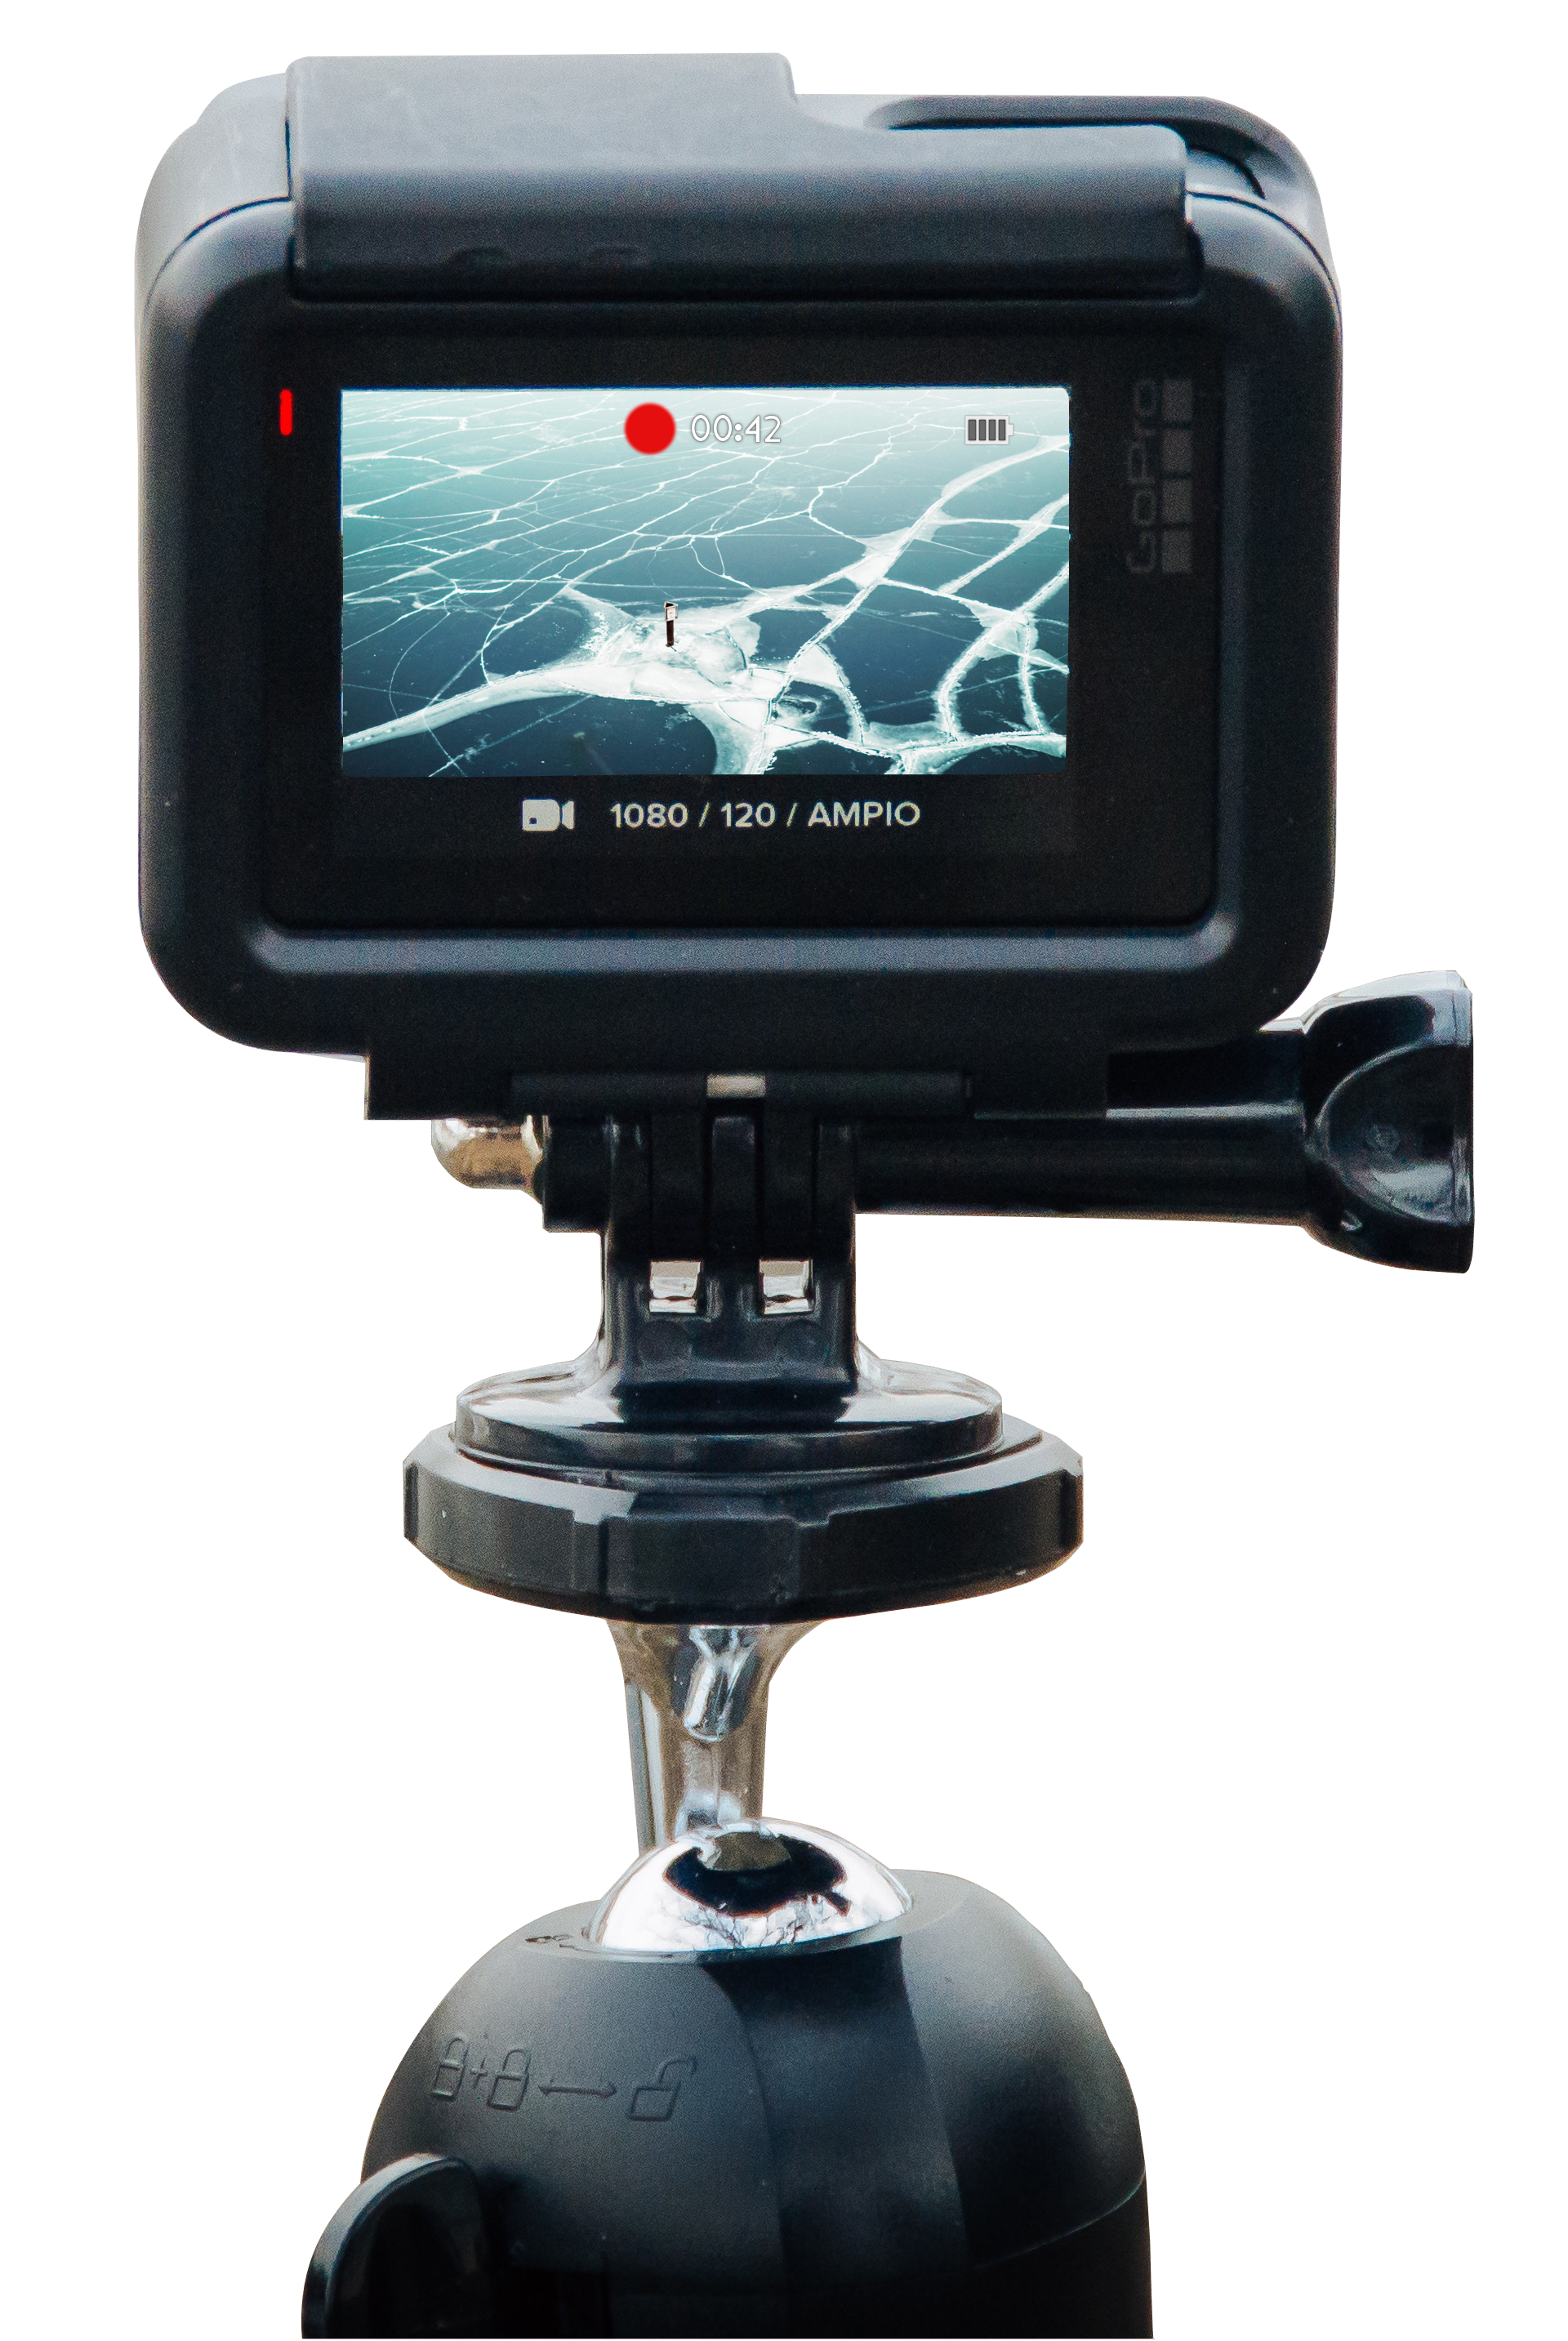
\includegraphics[width=0.7\linewidth]{images/tom-barett_fabrizio-verrecchia_unsplash-1x.png}
\end{figure}
% There is an offset of: .2 + .5 + .5 + 1 = 2.2 so take that into consideration (e.g. 4.74 - 2.2)
% 4.74 - 0.7 
% 2 - 0.81

\vspace{-1.5cm}
{\large{Melvin Richy Roest}}
\vspace{1cm}\\
\textsc{Vrije Universiteit Amsterdam} \\
Faculty of Sciences\\ 
Amsterdam, The Netherlands 2018

\renewcommand{\familydefault}{\rmdefault} \normalfont % Reset standard font

\end{titlepage}


% BACK OF COVER PAGE (BLANK PAGE)
\newpage
\restoregeometry
\thispagestyle{empty}
\mbox{}


% TITLE PAGE
\newpage
\thispagestyle{empty}
\begin{center}
	\textsc{\large Master's thesis 2018}\\[4cm]		% Report number given by department 
	\textbf{\Large } Exploring hypermedia in 2018 through the lens of XIMPEL\\[1cm]
	{\large Implications on parallel media, frustration detection and choice}\\[1cm]
	{\large Melvin Richy Roest}
	
	\vfill	
	% Logotype on titlepage	
	\begin{figure}[H]
	\centering
	% Remove the following line to remove the titlepage logotype
	\includegraphics[width=0.6\linewidth]{images/vu_logo.png} \\	
	\end{figure}	\vspace{5mm}	
	
	Department of Computer Sciences\\
	\emph{Section: Business Web \& Media}\\
	\textsc{Vrije Universiteit Amsterdam} \\
	Amsterdam, The Netherlands 2018 \\
\end{center}


% IMPRINT PAGE (BACK OF TITLE PAGE)
\newpage
\thispagestyle{plain}
\vspace*{4.5cm}
Exploring hypermedia in 2018 through the lens of XIMPEL\\
Implications on parallel media, frustration detection and choice\\
Melvin Richy Roest \setlength{\parskip}{1cm}

\copyright ~ Melvin Richy Roest, 2018. \setlength{\parskip}{1cm}

Supervisor and 1\textsuperscript{st} reader: Prof. Dr. Anton Eli\"ens\\
2\textsuperscript{nd} reader: Dr. ing. Sander C.J. Bakkes\\
Technical Supervision: Msc. Winoe Bhikharie\\
\setlength{\parskip}{1cm}

Master's Thesis 2018\\	% Report number given by department 
Department of Computer Sciences\\
Section: Business Web \& Media\\
Vrije Universiteit Amsterdam\\
De Boelelaan 1105, 1081 HV Amsterdam\\
Telephone +31 20 598 9898 \setlength{\parskip}{0.5cm}

\vfill
% Caption for cover page figure if used, possibly with reference to further information in the report
Cover: A visual metaphor for exploring the intersection between choice and media. The camera is cropped with the pen tool in Sketch 3. It comes from a from a beautiful photograph made by Fabrizio Verrecchia. The image in the camera is cropped from an epic background figure shot by Tom Barrett. \href{http://www.unsplash.com}{Unsplash.com} is the website where these beautiful gems have been found. The camera icons (record icon, time icon and battery icon) are made by yours truly with the marvelous pen tool. \setlength{\parskip}{0.5cm}

Typeset in \LuaLaTeX \\
Printed by Melvin's printer in his home\\
Amsterdam, The Netherlands 2018

